\title{Empowering GIS Using Big Data}

\author{Mrunal Lalitmohan Chaudhary}
\affiliation{%
  \institution{Indiana University}
  \city{Bloomington} 
  \state{IN} 
  \postcode{47408}
  \country{USA}}
\email{mchaudh@iu.edu}


% The default list of authors is too long for headers}
%\renewcommand{\shortauthors}{G. v. Laszewski}


\begin{abstract}
Location is an important metric when it comes to data. Be it the data of a Retailer which wants to analyze the customer behaviour in a given demography, or the Policemen who want to look into a particular crime committed in a given region, or tracking down a criminal's hideout, or a commercial giant wanting to figure out the ideal location for setting up a new plant to maximize their profits, location and geography play an important role. Knowing the geography can help immensely in generating more value in analysis, and in some extreme cases, like that of the census data of a country without the geography, the other data may prove to be meaningless. Since magnanimous amounts of data is getting generated every single second, at a break-neck speed, companies from across different domains, be it Insurance, Retail, Banking, Finance, Health care, Telecommunications, etc are quickly shifting to Big Data technologies from their traditional approaches. Thus it is an essential task to develop systems which empower the traditional Geographic Information Systems (GIS) with the Big data technologies to enhance the analysis and generation of insights.
\end{abstract}

\keywords{i523, HID205, GIS, Geospatial data, Geospatial data analysis}


\maketitle



\section{Introduction}
Location is an integral part of majority of the data sets and it plays an important role in the analysis. Spatial data is a numeric value that represents information about the location, size or shape of a physical object in the coordinate system \cite{link1}. Thus the position of a point in the coordinate system, location of a pond or a mountain on Earth, postal address of Indiana University, or the zip code of a region, etc. are all examples of spatial data. When such an information has a geographic aspect to it, it is called \emph{Geospatial data} \cite{link2}. The geospatial data is geo-referenced, meaning that the absolute or relative position of an object is decided in respect with Earth. This geospatial data is expressed in terms of longitudes and latitudes \cite{link1}. Spatial data can be of two forms:\\ (1) Vector: This data form uses points, line, polygons and other shapes to describe the spatial aspects like roads, streams, rivers or cities. \\ (2) Raster: This form stores data in the form of cells which represent the spatial features. Cities represent single cells, a road represent a linear sequence of cells and stream represent a collection of adjacent cells. Remote satellite data is one such example of raster \cite{link2}.\\
Though the term geospatial and GIS are used interchangeably, they are distinctively different. Geographic Information Systems (GIS) are a technological field that stores geographic information in layers and integrates it with geographic software programs in order to create, store, map, manipulate and analyze real world data \cite{link3}. GIS has the ability to to assemble the geospatial data into a systematic set of layers of maps thus disintegrating the complex themes to simplify analysis. All this data which contains information that is precise to its location on earth surface is enabled by layering. Hence it is termed as \emph{geospatial} \cite{link6}. 

\section{Background}
Since the last few years, the position and location of people along with their demographics; i.e geospatial data is gaining a lot of recognition because it has widespread applications in the field of analytics. For example, geospatial data is an imperative information that is needed by law enforcement agencies to predict and prevent crimes from happening by linking the crime rates of a particular crime with the location and thereby figuring out the reasons for that crime being rampant in a given geographic location \cite{link4}. Geospatial data can be used by Realtor and Commercials for pricing a property or discerning the ideal location for opening a new outlet through proximity analysis\cite{link5}. Google Maps is another excellent example of application of GIS. It can also be used fro predicting the outbreak of a disease or occurrence of a natural calamity \cite{link5}. Thus the use cases of geospatial data are widespread, varied and also those which deal with real time mammoth sized data. 
Though the first known usage of the term GIS was done in the early sixties, the traditional GIS systems are insignificant when it comes to analytics through meaningful interpretations \cite{link13}. Since the advent of advanced technologies like cloud, embedded systems, mobile and social media, the traditional ways of GIS operations like mapping and analysis have been rendered to be insufficient \cite{link5}.
When Osama Bin Laden was traced in 2011 through big data analysis that captured spatio-temporal data in real time to pinpoint his exact location, big data made headlines \cite{link10}. Since then, pioneers like the Esri extended the potential of GIS across the big data technologies to produce significant insights in trends, relations and patterns to a granular level in a spatial context \cite{link5}.

\section{The Three V's of Big Data}
Like other technologies which deal with a humongous amount of data, GIS transformed Big Data must also respond to the 3 Vs, namely Volume, Velocity and Variety:
\begin{itemize}
    \item Volume: Geospatial data consists of images and data collected from across the entire globe through remote sensors and satellites. This data is therefore voluminous in nature.
    \item Velocity: The satellite imagery captures data every second, of every day. Thus the data is real time and gets generated very fast.
    \item Variety: The data available from the different geospatial technologies is in the form of videos, images, data as well as in two dimensional and three dimensional coordinate systems. Thus there is a lot of variety in the format and this is very different than the conventional big data formats of either pixels or alphanumeric characters \cite{link9}.
\end{itemize}

\section{Sources of Spatial data}
There is a variety of technologies available which can collect spatial big data such as: \\
(1) Remote Sensing: Images, up to clarity of a meter, and data either from satellites or from airborne cameras or drones can be collected using Remote Sensing. This can be used for monitoring abuses done against human rights.\\
(2) Geographic Information Systems (GIS): GIS consists of number of tools for mapping and analyzing geospatial data to detect patterns and clusters in data, such as predicting outbreak of diseases.\\
(3) Global Positioning System (GPS): This is a network of U.S Department of Defense satellites which gives accurate location coordinates of physical objects or human beings to civilians and military personnel \cite{link6}.

\section{Role of Big Data in Maximizing the Spatial analysis}
Big data helps in carrying out efficient operations on data in minimal amount of time, thereby adding great value to the business and sustainable practices \cite{link10}. Following are the ways in which Big Data has empowered and enhanced the analysis of Geospatial data:
(1) Big data is capable of doing analysis of unstructured data like emails, blogs, meteorological data, etc in real time. This is extremely useful for analysis of location in retail, security, finance, etc.
(2) Big data helps in finding spatial relationships in data by seeing the geospatial data on a map, thereby adding a new dimension to problem solving and making sense of big data.
(3) Big data integrates multiple layers of the geospatial data for a clearer context, and the data in different formats captured by the system is analyzed by big data technologies to give a complete picture.
(4) The integration of big data with mapping results in getting deeper insights, profitability, better understanding of customer base, and easier visualization.
(5) Big data enables in case-by-case query processing and data mining of huge spatio-temporal data \cite{link10}.

\section{GIS Analysis for Big data}
As was discussed in the previous parts, location is an important attribute of any data for understanding and predicting trends. Hence many tools are available in the market which do geospatial big data analysis using different big data technologies. One such toolkit is developed by GIS tech giant, International Supplier of Geographic Information (Esri), which uses the Hadoop framework's distributed processing to analyze geospatial data \cite{link7}.
The main six tasks performed in the analysis of a general purpose GIS are
\begin{itemize}
    \item Cleaning Input data
    \item Map making
    \item Manipulation of data
    \item File management
    \item Query and analysis
    \item Visualization of results \cite{link8}
\end{itemize}

The GIS tools using the Hadoop framework perform these steps in the following manner: \\
(1) Aggregate the operations on every single record of spatial big data based on location through running filters.\\
(2) Define new areas which are represented by polygons and implement polygon analysis on the records.\\
(3) The analysis reports can be visualized on maps by implementing informative symbology.\\
(4) Once these maps are generated, a report can be published after the maps are integrated in it \cite{link7}. 

\subsection{Overview of the GIS for Hadoop toolkit}
The GIS for Hadoop toolkit consists of four libraries that processes and analyzes the Spatial big data. These libraries are as follows: \\
(1) The building block - Esri Geometry API for Java: This library consists of geometry objects, spatial operations and spatial indexing. Customized MapReduce applications can be built by deploying this library in Hadoop using Java.\\
(2) The framework - Spatial framework for Hadoop: This library is built upon the Esri Geometry API and enables users to define user functions which extend the capabilities of Hive. Thus users can manipulate data through implementing queries using the Hive Query Language (HQL). 
(3) The Connector - Geoprocessing Tools for Hadoop: This library basically acts as a connector between the ArcGIS and Hadoop. It enables conversion of data to and from the JSON format, submit the HQL workflows and transport the results generated by Hadoop into ArcGIS for visualization.The ArcGIS platform can be used extensively for publishing the maps online.
(4) The toolkit - GIS Tools for Big Data: This library integrates the above three into one toolkit. It consists of samples that aid in testing the deployment of these libraries with Hadoop and Hive. It also consists of instructions to ensure everything runs without any issues \cite{link7}.

\section{Case Study- Detecting Ebola outbreak using Geospatial Big Data}
Nearly 5000 people had died and more than 13000 people had been infected by the outbreak of the Ebola disease in the July of 2011. And if severe actions weren't taken Ebola would have claimed much more lives in some parts of Africa \cite{link11}.This was the biggest outbreak of Ebola since the identification of the disease in the early seventies \cite{link11}. Clearly immediate action had to be taken up. At this critical juncture, many Big data Analytics firms came forward to help Africa in combating this outbreak. Much of the focus was laid on the data collected from cell phone networks since they were well developed in Africa \cite{link12}. The American Red Cross Organization came forward with its GIS program and urged volunteers to help create a detailed map of some of the rural towns since some isolated areas in Africa lacked sign posts and didn't have a GPS connect. Thus mapping tools proved to be critical since they helped not only in tracking which cities were infected by it, but also in predicting spread of the disease to different locations. A website was developed which helped in tracking the infectious disease all around the world \cite{link11}.
Similar to Red Cross, IBM came forward and donated its softwares to the Government of many countries to capture, process, analyze and broadcast information generated from the insights drawn in the analysis. The IBM system was developed in collaboration with Airtel, a mobile operator company which set up phone numbers for the citizens to message and call to inform about the state of disease in their locations. The data from the mobile cell phone towers was captured, and then anonymized by a start-up, Echo mobile. Thus after analyzing the data, heat maps were generated which showcased the areas worst hit by the disease and predicted the locations that were possibly going to be infected by it \cite{link11}.
The GIS giant, Esri coordinate with U.S Centers for Disease Control collected data from the cell towers and plotted them in their own GIS softwares \cite{link11}.
Though the state then of data collection in Africa was still in the primitive form, and without a full fledged Geographic Information System, Big data analysis was helpful in predicting the future course of the disease, and with it, saving many lives \cite{link12}.

\begin{figure}
	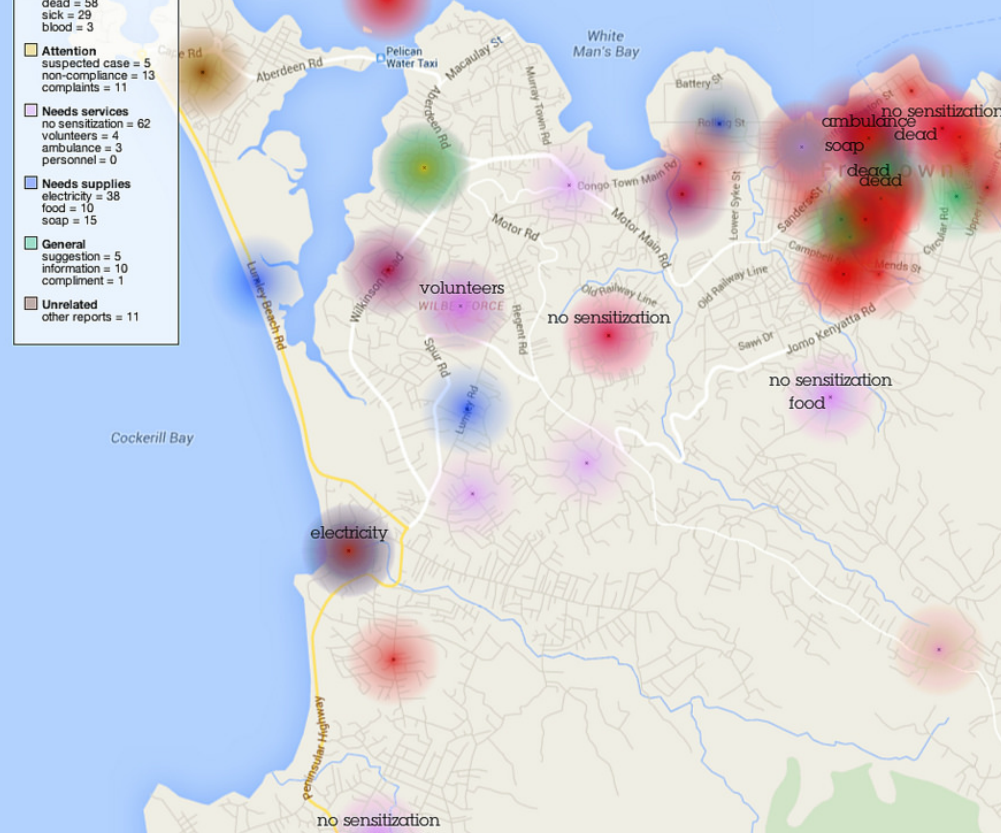
\includegraphics[width=\columnwidth]{images/ebola-heat-map.png}
	\caption{Heat map of Ebola cases generated by IBM based on cell phone data \cite{link12}}
	\label{F:heatmap}
\end{figure}
Figure \ref{F:heatmap} Shows heat map of Ebola cases generated by IBM based on cell phone data.\\

\section{Conclusion}
The Geographic Information Systems (GIS) help in answering two very crucial questions of \emph{when} and \emph{where} in analysis. Only after answering these questions can the \emph{how} and the \emph{why} of the customer behaviour, insurance frauds, business loss, etc can be answered, since human behaviour is entirely dependent upon the two parameters of space and time. Without the use of Big Daat, GIS is useful in having a very specific analysis. And without geospatial data, analysis is incomplete. GIS is detrimental to analysis. Thus in the current world, Big Data and GIS are two parts of a whole. With the advent of Big Data, like everything else, GIS too has undergone a drastic change. Hence GIS is constantly evolving, right from its meaning, to functions to the uses. And this is the only beginning. With fully developed Geographic Information Systems, it is possible to predict disease outbreaks, occurrence of natural calamities, track criminals, find locations through Google Maps, etc. 


\begin{acks}

  The authors would like to thank Dr. Gregor von Laszewski for his
  support and suggestions to write this paper.

\end{acks}

\bibliographystyle{ACM-Reference-Format}
\bibliography{report} 
